\documentclass{article}
\usepackage{fullpage}

%load needed packages
\usepackage{graphicx}
\usepackage{array}
\usepackage{booktabs}
\usepackage[utf8]{inputenc}
\usepackage[T1]{fontenc}
\usepackage{url}
\usepackage[spanish]{babel} % Paquete para el idioma español
\usepackage{float}  % Necesario para [H]
\usepackage{listings}
\usepackage{xcolor}

\definecolor{codegreen}{HTML}{5AB2FF}
\definecolor{morado}{HTML}{AD88C6}
\definecolor{BG}{HTML}{EEEEEE}
\definecolor{azul}{HTML}{4D869C}
\definecolor{sqlblue}{HTML}{FF8C00} % Color para las palabras clave SQL

% Estilo para DDL
\lstdefinestyle{ddlstyle}{
	language=SQL,
	backgroundcolor=\color{BG},
	commentstyle=\color{codegreen},
	basicstyle=\ttfamily\small,
	keywordstyle=\color{azul},
	stringstyle=\color{morado},
	showstringspaces=false,
	breaklines=true,
	frame=shadowbox,
	numbers=left,
	numberstyle=\tiny\color{gray},
	captionpos=b,
}

% Estilo para SQL
\lstdefinestyle{sqlstyle}{
	language=SQL,
	backgroundcolor=\color{BG},
	commentstyle=\color{codegreen},
	basicstyle=\ttfamily\small,
	keywordstyle=\color{sqlblue}, % Color diferente para palabras clave SQL
	stringstyle=\color{morado},
	showstringspaces=false,
	breaklines=true,
	frame=shadowbox,
	numbers=left,
	numberstyle=\tiny\color{gray},
	captionpos=b,
}

\begin{document}



% Portada
\begin{titlepage}
	\centering
	\vspace*{3cm}
	
	% Título destacado
	{\Huge \textbf{Diseño y Explotación de un almacén de 
			UCI Sanitaria}\\[0.5cm]}
	
	% Espacio y logotipo (si lo tienes, por ejemplo el logo de tu universidad)
	\vspace{2cm}
	
\includegraphics[width=0.3\textwidth]{images/uma_logo.jpg}\\[1cm]
	
	% Nombre del autor
	{\LARGE \textbf{Alejandro Silva Rodríguez}\\[0.5cm]}
	{\LARGE \textbf{Marta Cuevas Rodríguez}\\[0.5cm]}
	{\large \textit{Almacenes De Datos}\\
		Universidad de Málaga\\
		}
	
	\vfill
	
	% Fecha en la parte inferior de la página
	{\large Septiembre 2024}
\end{titlepage}

% indice
\tableofcontents

\newpage
\section{Introducción}
\label{sec:introduccion}

En el contexto hospitalario actual, el monitoreo y la gestión eficiente de los recursos es una necesidad apremiante, especialmente en unidades como la de Cuidados Intensivos (UCI), donde la administración de medicamentos representa una parte sustancial de los costos. A nivel mundial, el incremento en el costo de los medicamentos y la presión financiera sobre los sistemas de salud han impulsado la búsqueda de soluciones que optimicen el uso de los recursos en entornos críticos. Sin embargo, muchas instituciones hospitalarias carecen de herramientas analíticas específicas para monitorizar y analizar de manera detallada el gasto en fármacos, lo que limita la capacidad de identificar patrones de consumo y optimizar la asignación de presupuestos.\\

En Estados Unidos, la situación es especialmente significativa debido a la gran cantidad de recursos destinados a la atención en las UCI y la disponibilidad de grandes volúmenes de datos clínicos. Actualmente, existen bases de datos como la proporcionada por el Instituto de Tecnología de Massachusetts (MIT) \cite{eicu_crd}, que recogen información completa sobre los tratamientos, síntomas y diagnósticos de los pacientes, ofreciendo una oportunidad para profundizar en el análisis del gasto en medicamentos en pacientes críticos. No obstante, estas bases de datos no están estructuradas para un análisis enfocado exclusivamente en los costos de los medicamentos en el entorno de la UCI, lo que representa un vacío que este proyecto busca abordar.

\section{Objetivos}
\label{sec:objetivos}

Este proyecto tiene como objetivo desarrollar un almacén de datos específicamente diseñado para analizar el gasto en medicamentos en pacientes ingresados en la UCI en hospitales de EE.UU. A partir de la base de datos proporcionada por el MIT, se creará un modelo que permita identificar patrones de consumo y gasto en fármacos administrados a pacientes críticos. Con esto, se espera ofrecer una herramienta que aporte información valiosa para la gestión de recursos en las UCI, contribuya a optimizar los tratamientos y ayude en la planificación presupuestaria de los hospitales.

\section{Diseño Conceptual}
\label{sec:diseno_conceptual}

\subsection{Descripción del Modelo Conceptual}

El modelo conceptual de nuestro almacén de datos toma como hecho principal el \textbf{Gasto en Medicamentos} en la UCI del hospital, y como medidas las variables de \textbf{cantidad de gasto}, \textbf{tasa de infusión} y \textbf{volumen de fluido administrado}.

\begin{figure}[H]
	\centering
	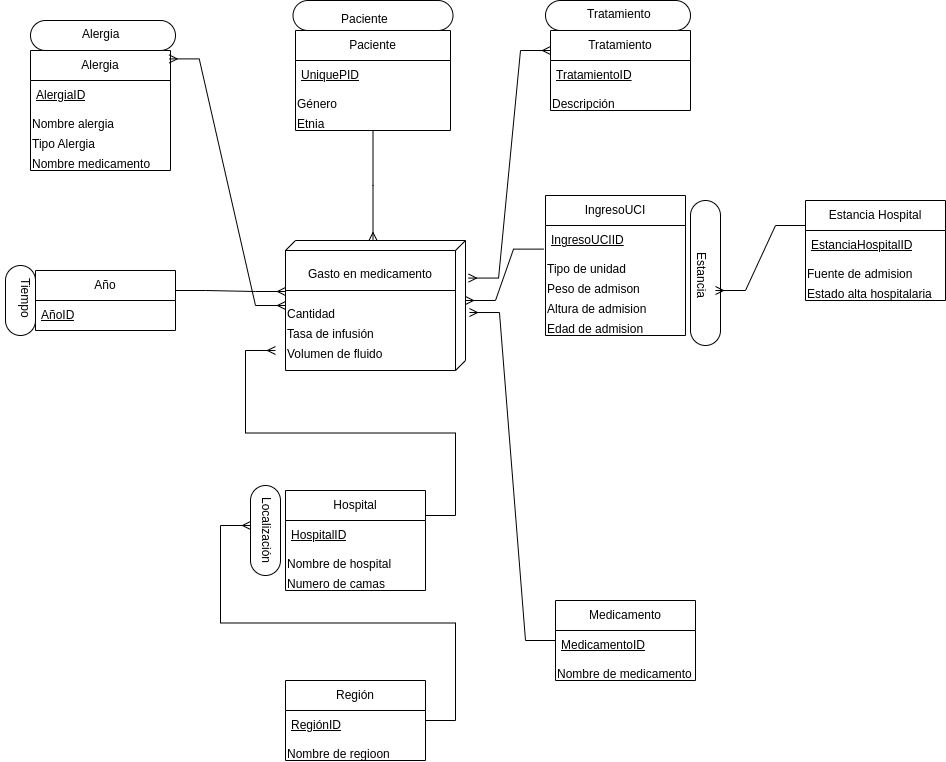
\includegraphics[width=.7\textwidth]{images/diseño_conceptual.png}
	\caption{Modelo Conceptual}
	\label{fig:conceptual}
\end{figure}


El modelo está compuesto por cinco dimensiones, descritas a continuación:

\begin{enumerate}
	\item \textbf{Tiempo}: Esta dimensión organiza los datos temporalmente mediante el atributo \textit{Año}.
	
	\item \textbf{Hospital}: La dimensión \textit{Hospital} incluye los niveles \textit{Región} y \textit{Hospital}, lo que permite agrupar los datos por área geográfica y hospital específico. Además, el hospital contiene como atributo una variable categórica que indica el número de camas (por ejemplo, <500 camas).
	
	\item \textbf{Estancia}: La dimensión \textit{Estancia} describe el tiempo de permanencia del paciente en el hospital. Está estructurada en los niveles \textit{Ingreso en UCI} y \textit{Estancia en el Hospital}, ya que un mismo paciente puede ingresar varias veces en la UCI durante una sola estancia en el hospital. Para el nivel \textit{Ingreso en UCI}, los atributos incluyen \textit{Tipo de Unidad}, \textit{Peso}, \textit{Altura}, \textit{Edad de Admisión} y \textit{Género del Paciente}. En cuanto a la \textit{Estancia en el Hospital}, los atributos incluyen la \textit{Fuente de Admisión} (departamento donde fue admitido) y el \textit{Estado de Alta Hospitalaria} (indicando si el paciente fue dado de alta vivo o fallecido).
	
	\item \textbf{Medicamento}: Esta dimensión permite categorizar los datos según el \textit{Medicamento} administrado al paciente en la UCI.
	

	\item \textbf{Tratamiento}: Esta dimensión clasifica el gasto en medicamentos según el tipo de \textit{Tratamiento} para el que se administran, permitiendo analizar el consumo de fármacos en función de las diferentes intervenciones clínicas en la UCI.
	
	\item \textbf{Alergia}: Esta dimensión agrupa los datos según los tipos de \textit{Alergias} presentes en los pacientes, indicando la relación entre las alergias y los medicamentos administrados, lo cual permite analizar cómo estas condiciones impactan en el gasto en fármacos.
	
	\item \textbf{Paciente}: Esta dimensión identifica al \textit{Paciente} en quien se produce el gasto de medicamentos, permitiendo un análisis individualizado del consumo de fármacos en función de las características demográficas y clínicas de cada paciente.
\end{enumerate}



\section{Diseño Lógico}
\label{sec:diseno_logico}
\subsection{Transformación a Modelo en Copo de Nieve}
Para construir el modelo lógico a partir del modelo conceptual, se realizó una transformación en la que cada dimensión y el hecho principal, \textbf{Gasto en medicamentos}, fueron convertidos en entidades relacionales en forma de tablas. El modelo lógico mantiene la estructura planteada en el modelo conceptual, permitiendo almacenar el gasto en medicamentos junto a los atributos de las diferentes dimensiones relevantes para el análisis.



\begin{figure}[H]
	\centering
	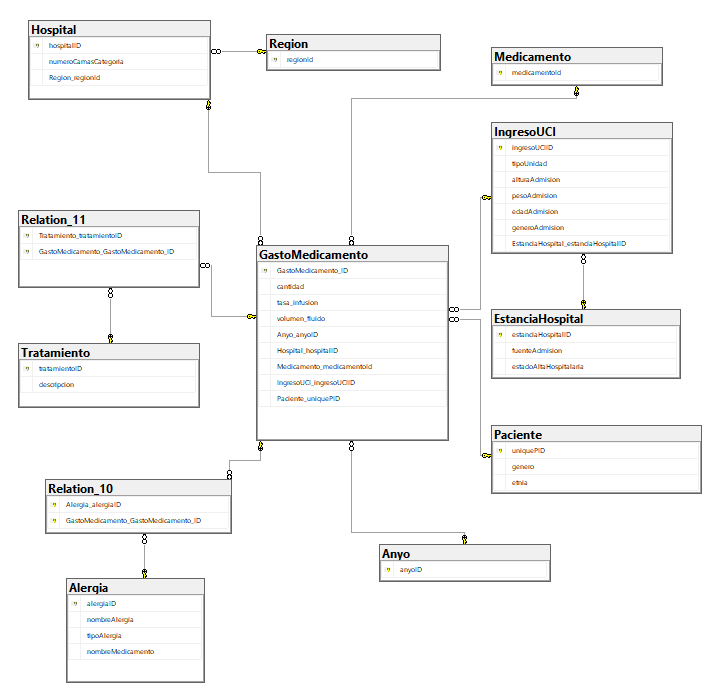
\includegraphics[width=.7\textwidth]{images/diseño_logico.png}
	\caption{Modelo Lógico}
	\label{fig:logico}
\end{figure}
Cada dimensión del modelo conceptual (\textit{Paciente}, \textit{Año}, \textit{Hospital}, \textit{Ingreso}, \textit{Medicamento}, \textit{Alergia} y \textit{Tratamiento}) se transformó en una tabla individual en el modelo lógico. Las tablas de dimensión incluyen sus atributos clave, manteniendo las jerarquías definidas en el modelo conceptual. La tabla central \textbf{GastoMedicamento} representa el hecho principal del modelo y contiene las medidas de análisis, como \textit{cantidad}, \textit{tasa de infusión} y \textit{volumen de fluido}. Esta tabla se conecta con las tablas de dimensión mediante claves foráneas, que reflejan las relaciones entre las dimensiones y el hecho central en la estructura relacional. De este modo, el modelo lógico permite realizar consultas eficientes sobre el gasto en medicamentos con base en las características de cada dimensión.

Para gestionar la relación de \textbf{GastoMedicamento} con las dimensiones \textit{Alergia} y \textit{Tratamiento}, que pueden tener una asociación de tipo \textbf{muchos-a-muchos}, fue necesario introducir tablas intermedias. Estas tablas, denominadas \textbf{Relation\_10} (para la relación entre \textit{GastoMedicamento} y \textit{Alergia}) y \textbf{Relation\_11} (para la relación entre \textit{GastoMedicamento} y \textit{Tratamiento}), permiten descomponer la relación muchos-a-muchos en dos relaciones de uno-a-muchos. De esta manera, cada registro en \textbf{GastoMedicamento} puede asociarse a múltiples alergias y tratamientos sin redundancia de datos ni inconsistencias. Las tablas intermedias incluyen claves foráneas hacia \textbf{GastoMedicamento} y hacia las tablas \textit{Alergia} o \textit{Tratamiento}, asegurando la integridad referencial en estas relaciones.

\subsection{Definición de Claves}
En el modelo lógico, cada tabla de dimensión se ha diseñado con una clave primaria única, que permite identificar de manera exclusiva cada registro y facilita las consultas sobre datos específicos. Estas claves primarias son identificadores (como \textit{PacienteID}, \textit{HospitalID}, \textit{MedicamentoID}, entre otros) y garantizan la integridad de los datos dentro de cada tabla.
\\

La tabla de hechos \textbf{GastoMedicamento} utiliza, además, claves foráneas que apuntan a las claves primarias de las tablas de dimensión. Por ejemplo, \textit{Paciente\_uniquePID} se utiliza como clave foránea para enlazar la tabla de \textit{Paciente} con \textbf{GastoMedicamento}, y de forma similar se manejan las relaciones con \textit{Hospital}, \textit{Medicamento}, y las demás dimensiones. Las tablas intermedias \textbf{Relation\_10} y \textbf{Relation\_11} también incluyen claves foráneas hacia las tablas de dimensión \textit{Alergia} y \textit{Tratamiento}, respectivamente, migrando las claves primarias de estas dimensiones a dichas tablas intermedias para mantener la relación de muchos-a-muchos.
\\

Este uso de claves foráneas permite conectar el hecho del gasto en medicamentos con las distintas características de cada dimensión, proporcionando una estructura organizada y facilitando la integridad referencial en el almacén de datos. Al tener un esquema de este tipo, el modelo se encuentra normalizado y optimizado tanto para la integridad de los datos como para mejorar la eficiencia en las consultas.

\subsection{Instrucciones para Crear el Almacén}
Proporciona una guía para desplegar el almacén de datos en SQL Server usando el código DDL, detallando los pasos a seguir y cualquier configuración de permisos o ajustes adicionales.

\section{Dificultades Encontradas}
\label{sec:dificultades_encontradas}
Enumera y describe las dificultades enfrentadas durante el desarrollo del proyecto. Explica cómo se resolvieron estos problemas o, en caso de no haber encontrado complicaciones, indícalo claramente.

\section{Conclusión}
\label{sec:conclusion}
Resumen de los principales resultados del proyecto, con un breve comentario sobre la utilidad del almacén de datos desarrollado y cómo este se alinea con los objetivos de la asignatura.


\newpage
\section{Acceso al Repositorio}

Toda la información adicional, incluyendo el código fuente y la documentación completa de este proyecto, está disponible en el repositorio de GitHub \cite{silva2024github}.

% Incluir la bibliografía
\bibliographystyle{plain}  % Estilo de la bibliografía (por ejemplo, plain, alpha, ieee, etc.)
\bibliography{bibli}  % Nombre del archivo .bib sin la extensión

\end{document}
